%% IDE has R L T A 3
%% timetable has L R A 3
\documentclass[12pt,a4paper,twoside]{article}
\usepackage{graphicx,fancyhdr}
\pdfpagebox=4

\setlength{\parindent}{0cm}
\setlength{\parskip}{2ex plus1ex minus 0.5ex}

\addtolength{\evensidemargin}{-2.5cm}
\addtolength{\oddsidemargin}{-0.5cm}
\addtolength{\textwidth}{3cm}

\addtolength{\headheight}{0.2cm}
\addtolength{\topmargin}{-2.5cm}
\addtolength{\textheight}{2.5cm}

% \newcommand{\source}[1]{\textbf{\verb^#1^}}}
\renewcommand{\_}{\texttt{\symbol{95}}}
\addtolength{\fboxsep}{0.1cm}
\newcommand{\param}[1]{\textit{\textrm{\textmd{#1}}}}
\newcommand{\codebar}{\rule{\textwidth}{0.3mm}}
\newcommand{\todo}{\textbf{TODO}}

\newlength{\codelen}
\newcommand{\code}[1]
{\begin{center}\fbox{\parbox{16cm}{\texttt{#1}}}\end{center}}

\newcommand{\mission}[1]{\item[#1:]}
% \newcommand{\mission}[1]{\texttt{#1}\hspace{3mm}}

\fancyhead{}
\fancyhead[RO,LE]{\thepage}
\fancyhead[LO,RE]{Tealight Summer School Exercises}
\fancyfoot{}
\pagestyle{fancy}
% \pagestyle{empty}

\setcounter{secnumdepth}{1}

\newenvironment{bulletlist}
{
	\begin{itemize}
	\addtolength{\itemsep}{-1mm}
	% \setlength{\itemsep}{0ex}
	\setlength{\parsep}{0ex}
}
{
	\end{itemize}
}

\newenvironment{alphalist}
{
	\begin{enumerate}
	\setlength{\itemsep}{0ex}
	\setlength{\parsep}{0ex}
	\renewcommand{\labelenumi}{(\alph{enumi})}
}
{
	\end{enumerate}
}

\newenvironment{numericlist}
{
	\begin{enumerate}
	\addtolength{\itemsep}{-1mm}
	% \setlength{\itemsep}{0ex}
	\setlength{\parsep}{0ex}
}
{
	\end{enumerate}
}

\usepackage{hyperref}
\begin{document}

\centerline{\textbf{\LARGE Tealight Summer School Exercises}}
\vspace{0.5cm}
\centerline{August 2015}
\centerline{Author: Ian Davies}
\centerline{Based on ROBOC exercises by David Eyers (\texttt{David.Eyers@cl.cam.ac.uk})}

{ \parskip 1mm plus 1pt \tableofcontents }

\newpage
\section{Logo Mode} \label{sec:logo-mode}

\subsection{Exercises}

\begin{numericlist}
\item Run the spiral program.
	Change the angle from 90 to 91 degrees and test what difference
	this makes. Can you explain how the program works?
\item Run the polygon program, then modify it to draw a circle.
\item Run the waterwheel program. Change it to make the paddles on the
	waterwheel triangular.
\item Write a program to draw a chessboard.
\item Run the fractal snowflake program. Try changing the detail parameter of the segment function. Write similar programs to produce the trangle fractal and tree fractal shown in Figure \ref{fractal}. 

\end{numericlist}

\begin{figure}[h]
\centering
%\fbox{
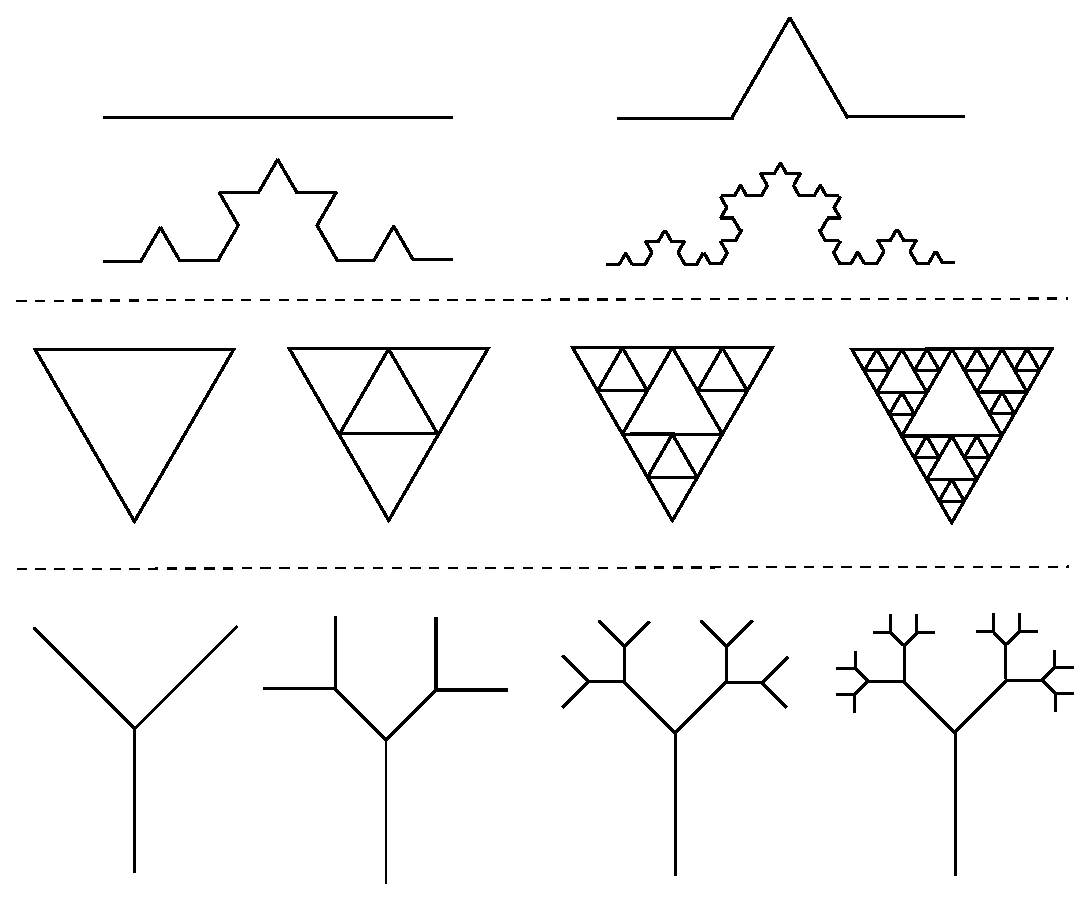
\includegraphics[scale=0.5,trim=10mm 10mm 10mm 155mm]{diagrams/new_fractal}
%}
\caption{Levels of detail for snowflake, triangle and tree fractals}
\label{fractal}
\end{figure}

\newpage
\section{Robot Mode}\label{sec:robot-mode}

\subsection{Some ideas}

\begin{bulletlist}
\item Use \verb^left_side()^ and \verb^right_side()^ to spot fruit or turn
	into a side passage
\item To turn alternately left or right, create a variable called \verb^dir^
	(for example) and change it from \verb^-1^ to \verb^1^ each time you turn:
	\begin{verbatim}
	dir = 1
	#...
	turn(dir)
	dir = -dir
	\end{verbatim}
\item Use senses to work out when you are in a dead end and then turn around
\item Spin around on the spot checking for fruit ahead with \verb^look()^
\item Use a counter variable to take an action every \verb^k^ steps
\item Keep track of the distance travelled or the direction you are
	facing, and use this to change the robot's behaviour
\end{bulletlist}

\subsection{Hints for missions}

\begin{description}
\mission{SEARCH}
	Avoid a pre-planned route---use sensors instead to alert the robot to
	nearby targets. If you can hit ten targets your robot passes
	this mission. Expert programmers might be able to find thirty or more!

\mission{CHESS}
	The grid pattern is fixed and regular, so this time you don't need to
	use sensors to tell you where to go.
	Instead you will need to plan your route carefully to trace over the
	lines, and write loops to avoid repeating steps in your program.

\mission{TRAIL}
	Use sensors and turn towards the footprints to make sure
	your robot stays on course.

\mission{CLEANUP}
	You need to use sensors to detect the edges of the pool.
	This is quite difficult to get right.

\mission{MAZE}
	This type of maze can be solved by
	following either the left or right wall.

\mission{MINE}
	Efficiency is key---you will only pass this test if you
	waste no time, gathering items almost continuously throughout the
	time allowed.

\mission{FIELD}
	Try to avoid walking in straight lines for long distances, when
	there may be flowers nearby.

\mission{TREASURE}
	The gems are found in clusters. Once you have found a
	gem, look around nearby for the rest of the cluster, then
	go exploring for the next set.

\mission{VINE}
	This challenge requires recursion and backtracking.

\end{description}

\newpage
\section{Art Mode}\label{sec:art-mode}

\subsection{Exercises}

\begin{numericlist}
\item Run the shapes program. Now make the spot a bit smaller, put the spot
		inside the circle and put the square under the circle.
\item Run the images program, then change the flower stripes to be horizontal
		instead of vertical. Next, make the stripes diagonal.
\item Run the stars program, then adapt it to draw ellipses instead.
\item Test the sketch program, and change it so that the right mouse
		button draws in a different colour.
\item Control the orbits program with the cursor keys, and try to keep the spot on the screen.
	Now add gravity to the program, and friction.
\end{numericlist}

\end{document}
